%%
%% This is file `sample-acmsmall-conf.tex',
%% generated with the docstrip utility.
%%
%% The original source files were:
%%
%% samples.dtx  (with options: `acmsmall-conf')
%% 
%% IMPORTANT NOTICE:
%% 
%% For the copyright see the source file.
%% 
%% Any modified versions of this file must be renamed
%% with new filenames distinct from sample-acmsmall-conf.tex.
%% 
%% For distribution of the original source see the terms
%% for copying and modification in the file samples.dtx.
%% 
%% This generated file may be distributed as long as the
%% original source files, as listed above, are part of the
%% same distribution. (The sources need not necessarily be
%% in the same archive or directory.)
%%
%% The first command in your LaTeX source must be the \documentclass command.
\documentclass[acmsmall, screen, nonacm]{acmart}
%% NOTE that a single column version is required for 
%% submission and peer review. This can be done by changing
%% the \doucmentclass[...]{acmart} in this template to 
%% \documentclass[acmsmall,screen,review]{acmart}
%% Or use the sample-acmsmall-submission.tex file.
%% 
%% To ensure 100% compatibility, please check the white list of
%% approved LaTeX packages to be used with the Master Article Template at
%% https://www.acm.org/publications/taps/whitelist-of-latex-packages 
%% before creating your document. The white list page provides 
%% information on how to submit additional LaTeX packages for 
%% review and adoption.
%% Fonts used in the template cannot be substituted; margin 
%% adjustments are not allowed.

%%
%% \BibTeX command to typeset BibTeX logo in the docs
\AtBeginDocument{%
  \providecommand\BibTeX{{%
    \normalfont B\kern-0.5em{\scshape i\kern-0.25em b}\kern-0.8em\TeX}}}

%% Rights management information.  This information is sent to you
%% when you complete the rights form.  These commands have SAMPLE
%% values in them; it is your responsibility as an author to replace
%% the commands and values with those provided to you when you
%% complete the rights form.
\setcopyright{acmcopyright}
\copyrightyear{2018}
\acmYear{2018}
\acmDOI{10.1145/1122445.1122456}

%% These commands are for a PROCEEDINGS abstract or paper.
\acmConference[Woodstock '18]{Woodstock '18: ACM Symposium on Neural
  Gaze Detection}{June 03--05, 2018}{Woodstock, NY}
\acmBooktitle{Woodstock '18: ACM Symposium on Neural Gaze Detection,
  June 03--05, 2018, Woodstock, NY}
\acmPrice{15.00}
\acmISBN{978-1-4503-XXXX-X/18/06}


%%
%% Submission ID.
%% Use this when submitting an article to a sponsored event. You'll
%% receive a unique submission ID from the organizers
%% of the event, and this ID should be used as the parameter to this command.
%%\acmSubmissionID{123-A56-BU3}

%%
%% The majority of ACM publications use numbered citations and
%% references.  The command \citestyle{authoryear} switches to the
%% "author year" style.
%%
%% If you are preparing content for an event
%% sponsored by ACM SIGGRAPH, you must use the "author year" style of
%% citations and references.
%% Uncommenting
%% the next command will enable that style.
\citestyle{acmauthoryear}

%%
%% end of the preamble, start of the body of the document source.
\begin{document}

%%
%% The "title" command has an optional parameter,
%% allowing the author to define a "short title" to be used in page headers.
\title{ANM project: DANM! team}

%%
%% The "author" command and its associated commands are used to define
%% the authors and their affiliations.
%% Of note is the shared affiliation of the first two authors, and the
%% "authornote" and "authornotemark" commands
%% used to denote shared contribution to the research.
\author{Aurelien Vu Ngoc}
% \authornote{Both authors contributed equally to this research.}
\email{vunaa10@mails.tsinghua.edu.cn}
% \orcid{1234-5678-9012}
% \author{G.K.M. Tobin}
% \authornotemark[1]
% \email{webmaster@marysville-ohio.com}
\affiliation{%
  \institution{Tsinghua University}
  \streetaddress{30 Shuangqing Rd}
  \city{Haidian Qu}
  \state{Beijing Shi}
  \country{China}}

% \author{Lars Th{\o}rv{\"a}ld}
% \affiliation{%
%   \institution{The Th{\o}rv{\"a}ld Group}
%   \streetaddress{1 Th{\o}rv{\"a}ld Circle}
%   \city{Hekla}
%   \country{Iceland}}
% \email{larst@affiliation.org}

% \author{Valerie B\'eranger}
% \affiliation{%
%   \institution{Inria Paris-Rocquencourt}
%   \city{Rocquencourt}
%   \country{France}
% }

% \author{Aparna Patel}
% \affiliation{%
%  \institution{Rajiv Gandhi University}
%  \streetaddress{Rono-Hills}
%  \city{Doimukh}
%  \state{Arunachal Pradesh}
%  \country{India}}

% \author{Huifen Chan}
% \affiliation{%
%   \institution{Tsinghua University}
%   \streetaddress{30 Shuangqing Rd}
%   \city{Haidian Qu}
%   \state{Beijing Shi}
%   \country{China}}

% \author{Charles Palmer}
% \affiliation{%
%   \institution{Palmer Research Laboratories}
%   \streetaddress{8600 Datapoint Drive}
%   \city{San Antonio}
%   \state{Texas}
%   \country{USA}
%   \postcode{78229}}
% \email{cpalmer@prl.com}

% \author{John Smith}
% \affiliation{%
%   \institution{The Th{\o}rv{\"a}ld Group}
%   \streetaddress{1 Th{\o}rv{\"a}ld Circle}
%   \city{Hekla}
%   \country{Iceland}}
% \email{jsmith@affiliation.org}

% \author{Julius P. Kumquat}
% \affiliation{%
%   \institution{The Kumquat Consortium}
%   \city{New York}
%   \country{USA}}
% \email{jpkumquat@consortium.net}

%%
%% By default, the full list of authors will be used in the page
%% headers. Often, this list is too long, and will overlap
%% other information printed in the page headers. This command allows
%% the author to define a more concise list
%% of authors' names for this purpose.
% \renewcommand{\shortauthors}{Trovato and Tobin, et al.}

%%
%% The abstract is a short summary of the work to be presented in the
%% article.
\begin{abstract}
  TODO: abstract, conclusion, related work and insert some figures + furnish round 2 solution part
\end{abstract}

%%
%% The code below is generated by the tool at http://dl.acm.org/ccs.cfm.
%% Please copy and paste the code instead of the example below.
%%
\begin{CCSXML}
<ccs2012>
   <concept>
       <concept_id>10003033.10003068</concept_id>
       <concept_desc>Networks~Network algorithms</concept_desc>
       <concept_significance>300</concept_significance>
       </concept>
 </ccs2012>
\end{CCSXML}

\ccsdesc[300]{Networks~Network algorithms}

%%
%% Keywords. The author(s) should pick words that accurately describe
%% the work being presented. Separate the keywords with commas.
\keywords{Advanced Network Management, Anomaly Detection, Time Series Outlier Detection}

%% A "teaser" image appears between the author and affiliation
%% information and the body of the document, and typically spans the
%% page.
% \begin{teaserfigure}
%   \includegraphics[width=\textwidth]{sampleteaser}
%   \caption{Seattle Mariners at Spring Training, 2010.}
%   \Description{Enjoying the baseball game from the third-base
%   seats. Ichiro Suzuki preparing to bat.}
%   \label{fig:teaser}
% \end{teaserfigure}

%%
%% This command processes the author and affiliation and title
%% information and builds the first part of the formatted document.
\maketitle

\section{Introduction}
This project aims to design a performant AIOps algorithm to take care of the troubleshooting of a given web service. 
This work includes taking into consideration the many complex call relations between each microservice and make good use of the various available performance indicators, all while being a live algorithm capable of reacting in real-time. 
This implies having the capacity to trace back in time the origin of potential anomalies before making precise and quick decisions to help the system recover, and also further develop abilities to recognize potential threats to prevent the system from failing at all. 
More specifically, this project focuses on pinpointing the anomalies when they happen and analyzes the provided data to find the root cause of the event. 

\section{Problem Background and Related Work}
Digitalization has come to a point where systems are fully interconnected with each other, thus relying on one another to perform as well as possible. 
Many systems are based on a microservice approach where each subcomponent has a very specific role inside the global work chain. 
Similar to an assembly line work in the 1900s, this method provides high performance because microservices are specialists at their own task while allowing a heavy global workload because all tasks can be achieved simultaneously.
\\
As appealing as this method can appear at first glance, it comes with some incoveniences and problems as well: the major concern is cascading microservice failures resulting in a global failure. 
In order to prevent the system from failing, companies were originally hiring system engineers to monitor and repair the system, but with the exponential growth of web services and their various microservices, it has become impossible to monitor all of them at once. 
That's where AIOps comes in to save the day, using artificial intelligence recent progress to make this monitoring task less tedious, more precise and eventually faster.
\\
% Many researches have been conducted to design optimal solutions to this kind of problem, reviews of the best methods are numerous as well. 
% \cite{nedelkoski_anomaly_2019}


\section{General Architecture}
First let's examine the architecture of the web service. 
Composed of multiple microservices with well-defined APIs that communicate, exchange and interact with each other, the web service produces 3 different kinds of data to deal with:
\begin{itemize}
  \item ESB business indicator data
  \item Trace data
  \item Hosts Key Performance Indicators (KPIs) data 
\end{itemize}
Through a Tencent Cloud Virtual Machine, our program is able to consume real-time data retrieved from a Kafka broker, to analyze these different sources of information as well as to detect anomalies and their root cause within 5 minutes after the anomaly occurrence. 
\\
Below we report our solution to this project for the different rounds of evaluation. 
During the first round, we tried to make use of the ESB data in order to discover anomalies, before analyzing the hosts KPIs to retrieve the source of the anomaly. 
Whereas in the second and third rounds, our approach was different and, learning from the other groups' presentations, we decided to switch to a method based on the analysis of the trace data to be more reactive. 
   


\section{Round 1 Solution}
This section explicits the details of the first round solution we implemented on the server. 
Unfortunately the final result is zero due to compatibility issues we encountered with the environment on the Tencent Cloud VM that we did not realize was causing our program to fail. 
An organizational problem within the team was a major factor in this miscalculation. 

\subsection{Anomaly Detection using Business Index}
The first step of this solution is to discover anomalies using ESB data, which can be achieved through multiple methods including an exponential moving average (EMA), and an unsupervised method specially developped for time series anomaly detection, HBOS (histogram based outlier detection \cite{goldstein_histogram-based_2012}). 
Both methods are extremely easy to implement, the former being the easiest because it does not require any model to be trained, only statistical consideration are required.
We decided this solution should preferably use the \verb|avg_time| feature of the ESB data, rather than the \verb|success_rate|, because unsuccessful business index are extremely rare and it does not help finding anomalies that much. 
Even though the HBOS approach showed promising results in the first place, we finally opted for the EMA method. 
EMA can be implemented effortlessly while being free from any dependencies (as opposed to HBOS which is not implemented in the standard python libraries).

% insert figures of anomaly detection with HBOS and EMA

\subsection{Candidate Anomalous Host}
Once our program correctly detected an anomaly, we needed to draw out candidate anomalous hosts for further testing and analysis. 
We used Trace data to complete this step by analyzing the call time of each node in the call chain graph using the \verb|elapsed_time| of each node. 

\subsection{Anomalous Key Performance Index Retrieval}
Originally, this step of retrieving the anomalous KPIs from the anomalous node was also trying to find the root cause. 
Finding anomalous behaviours in KPIs would lead to a ranking of the most "anomalous" behaviours that would later be flagged as the source host of the anomaly. 
However the results did not follow and we found that having the root cause analysis step provided better results. 
\\
\\
The core idea behind this first round's solution is to use machine learning models to predict KPIs values and compared them to the received KPIs values from the server. 
The difference between the true and the predicted value that would force the KPI into being considered anomalous, is measured using a predefined threshold on an error function. 
We tried various error functions, including: mean absolute error (MAE), mean relative error (MRE), mean squared error (MSE), binary cross-entropy.
\\
\\
The proper functioning of this step essentially resides in the choice of the model that will make such prediction. 
Since the problem deals with Time Series, there are many models indicated for this type of use including statistical methods (such as ARIMA and its multiple variants),  decision trees (such as XGBoost) or deep learning (such as LSTM based neural networks). 
Additionally, the methods detailed below require some data transformation and feature engineering. 
Incoming data from the server is modified into a "supervised dataset" where the input has columns for each KPI time series, further divided into past values (at times t-1min, t-2min, ...) and output has one columns for each KPI time series with only the current value (t). 
In order to tackle the missing values issue, we decided to go for forward-fill imputing because every KPI has different update frequency and we considered missing values as an absence of update, i.e. the value has not changed up until now.
\\
\subsubsection*{LSTM}
\begin{figure}[h!]
  \centering
  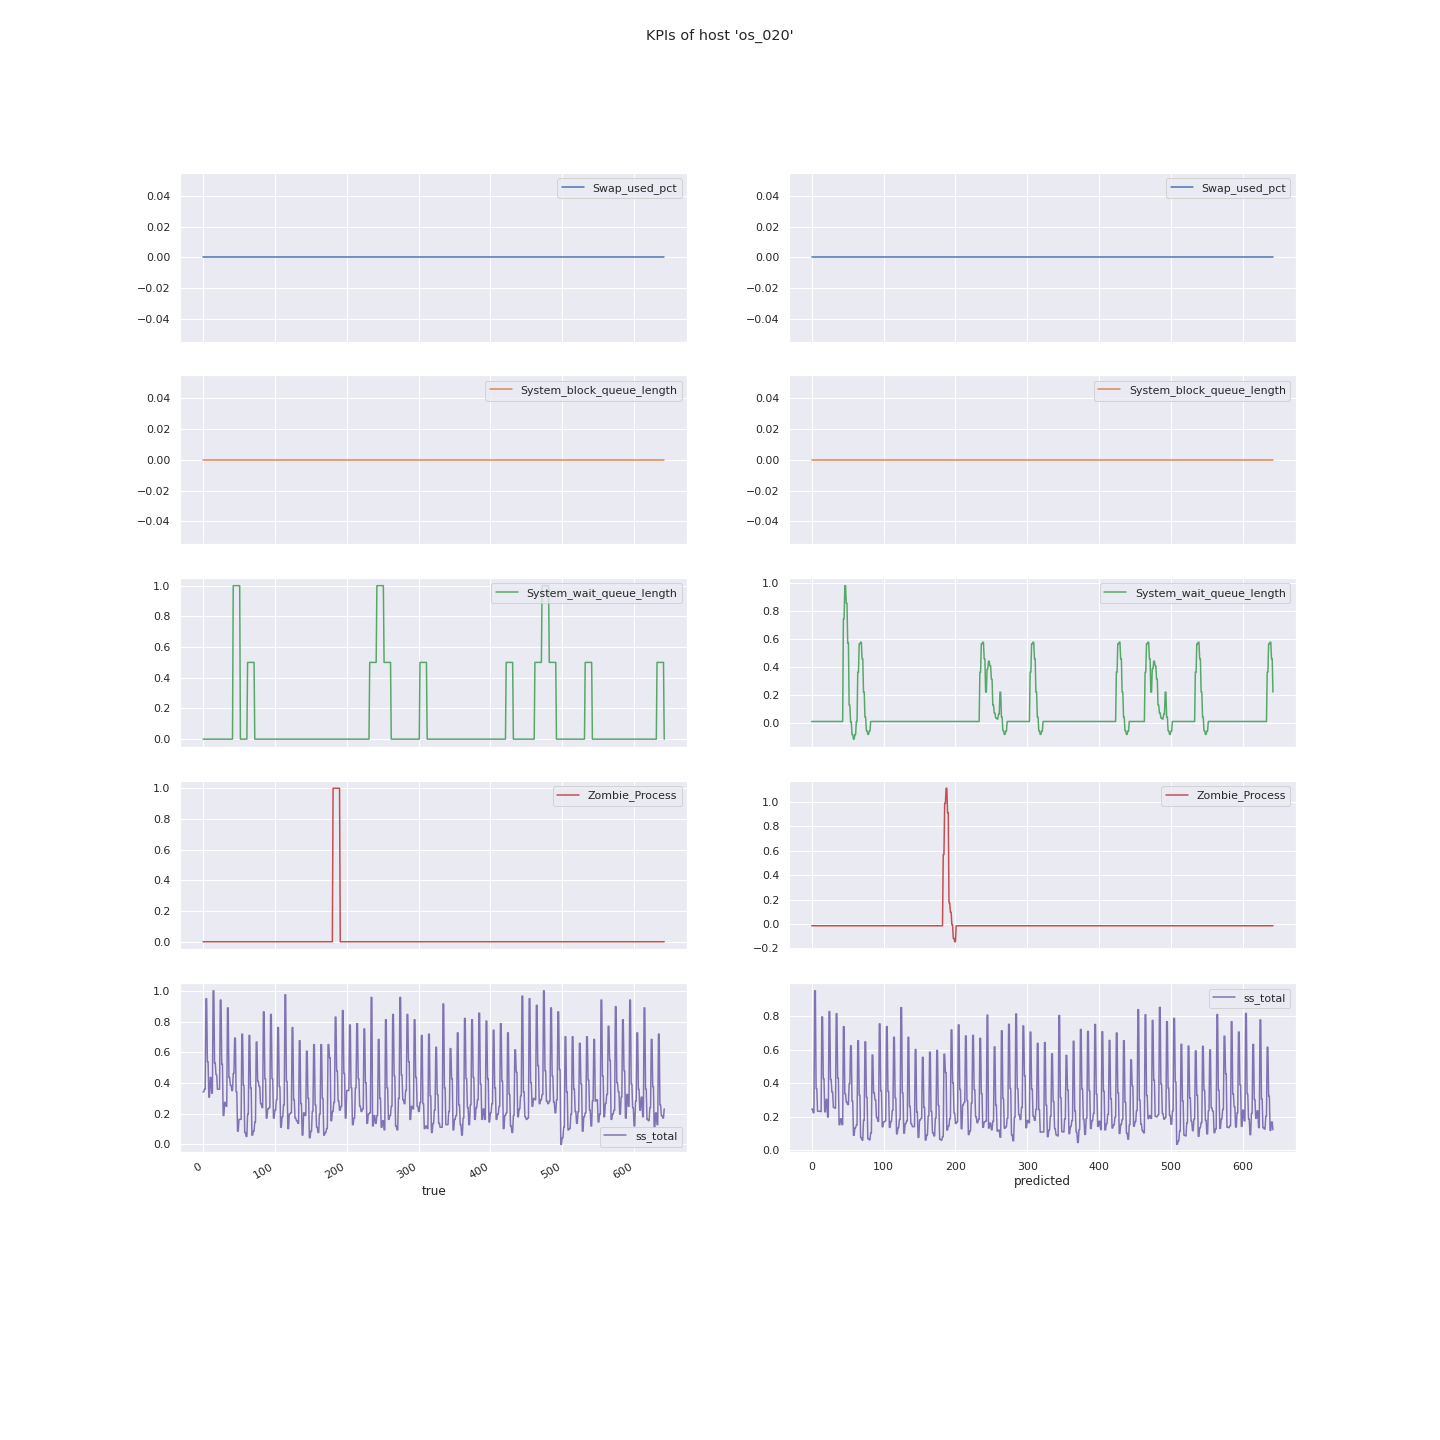
\includegraphics[width=0.5\textwidth]{images/lstm.png}
  \caption{Architecture of a LSTM model to forecast KPIs values of a given host (true/predicted)}
  \label{fig:lstm_architecture}
\end{figure}

Long Short Term Memory (LSTM) cells are optimal for time series prediction, in fact, a unique cell is capable of forecasting a time series with very high accuracy. 
Therefore using such a model on KPIs seems appropriate and we decided to assign one model to each host with each model composed of n independent cells in parallel, n being the number of KPIs describing the given host (see \autoref{fig:lstm_architecture}).
However, because LSTM need supervised datasets as input, we have to transform the time series dataset beforehand, which can be achieved through a succession of pandas operations on the data. 
\\
\begin{figure}[h!]
  \centering
  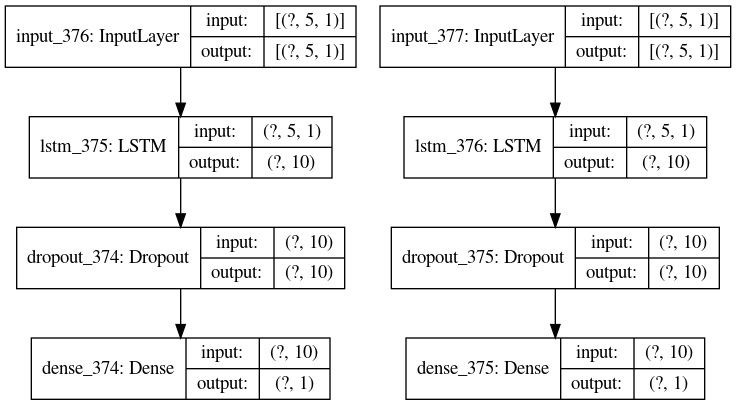
\includegraphics[width=0.5\textwidth]{images/lstm_model.png}
  \caption{KPIs: Time series forecasting using LSTM cells}
  \label{fig:lstm}
\end{figure}
In addition to this design, we also tried various LSTM architecture including Vanilla LSTM, stacked LSTM, CNN together with LSTM, but the single cell design was sufficient.
LSTM time series forecasting showed promising results that can be improved with further tuning and analysis (see \autoref{fig:lstm}). 
But this method was designed to work hand in hand with the candidate anomalous host step, that was lacking efficiency when it was implemented. 
In the sake of time and of simplicity, we decided to abandon this approach in the next rounds. 

\subsubsection*{XGBoost}
XGBoost is an extremely popular algorithm to solve structured supervised problems that have recently proven to be particularly effective, and rather simple to implement.
Again, the given problem does not label exactly as "supervised problem", so we had to transform the data to fit xgboost input.
Adapting xgboost to the given problem was also challenging because of the strategy to adopt: how many models do we need? 
Since xgboost cannot handle categorical data well \cite{chen_xgboost_2016} (e.g. host name, KPI name\dots), do we need to have a model for each? 
We came up with 2 solutions: use a multioutput wrapper for xgboost to support all hosts and KPIs at once, or switch to LightGBM.
Though we tried the multiple xgboost models approach as well as the multiouput single xgboost model approach, the results were not as promising as LSTM. 
\autoref{fig:xgboost} in \autoref{sec:appendix_xgboost} shows a sample of predicted kpis using the multioutput xgboost model where some predictions are not that accurate.

\section{Round 2 Solution}
This time around anomalies are detected using trace and host KPIs data only because the business index data has a low frequency update that can make the program skip anomalies. 
Inspired by the best solutions method, we switched back to a rule-based model.
A set of rules analyzes the trace data using different engineered features including: the \verb|elapsed_time| (that is natively inside the trace data), the \verb|call_time| of hosts (i.e. the time spent in edges of the trace call graph), the position of hosts in the call graph (child, parent, cousin) and their own features. 
% insert table with the engineered features
\\
Our program first compares the \verb|elapsed_time| of nodes with all-time recorded values and flags the host as anomalous if its value goes over a certain threshold (the 99.99\% quantile).
Then a second layer of tests using a z-score analysis inside a 20 minutes moving window ($zscore = (x-mean) / std$) can detect anomalies by comparing the computed z-score to a specific threshold determined using the training data.
Since the z-score gives an estimation of how far a value inside a series is from its mean (more specifically, how many standard devation away this value is from the mean), this indicator is easily interpretable and delivers good results. 
\\
Afterwards, there is a series of specific tests for particular configuration and well-defined anomalies such as "db close" error, "db connection limit" or "os network delay".
These errors have associated KPIs that are easily tractable: \verb|Sent_queue| and \verb|Received_queue| for the os anomalies ; \verb|On_Off_State| and \verb|tnsping_result_time| for the db faults. 
Sudden peaks have tremendous influence on the system and should be considered outliers. 
We monitored such peak events through a simple upper bound threshold determined using the training labeled data.  
\\
Then comes the engineered features. 
The core idea behind this approach is to find patterns in the fixed call chain graph that induces faults and errors. 
\autoref{fig:call_graph} shows how microservices call each other. 
This allows manual analysis using the labeled data to discover anomalous patterns, including:
\begin{itemize}
  \item high \verb|call_time| often implies a network issue (delay or loss), depending on the status of KPIs \verb|Sent_queue| and \verb|Received_queue|
  \item increasing incoming and outgoing \verb|call_time| often translates as an intern problem (such as CPU usage issue)
  \item \dots
\end{itemize}

\begin{figure}[h!]
  \centering
  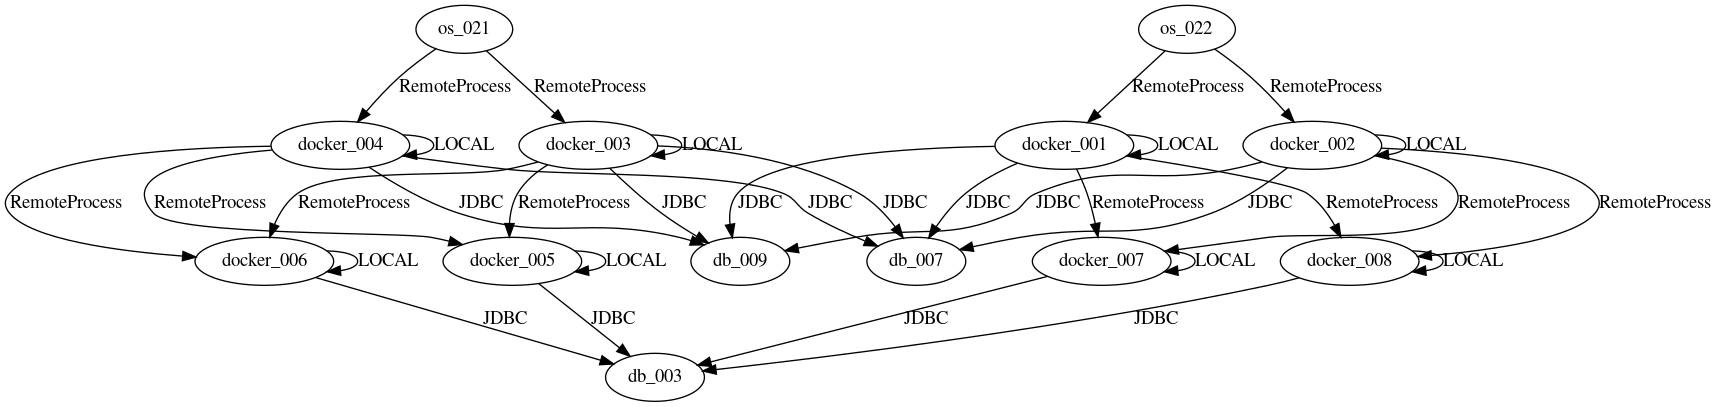
\includegraphics[width=\textwidth]{images/call_graph.png}
  \caption{The web service architecture has a fixed call graph.}
  \label{fig:call_graph}
\end{figure}


\newpage
\section{Work allocation}
\begin{table}[h!]
  \centering
  \begin{tabular}{|l|l|l|l|}
  \hline
               & \multicolumn{1}{c|}{Aurelien VU NGOC} & \multicolumn{1}{c|}{Fabien RAVET} & \multicolumn{1}{c|}{Aleksander} \\ \hline
  round 1      & HBOS, xgboost, LSTM                              & EMA for esb anomaly detection     &                                 \\ \hline
  round 2 \& 3 & Rule-based solution                              &                                   &                                 \\ \hline
  other        & This report, Tencent VM code design              &                                   &                                 \\ \hline
  \end{tabular}
  \caption{Project work allocation}
  \label{tab:work_allocation}
\end{table}

An insight of the work allocation can also be found in the GitHub commit history at the following url: \url{https://github.com/DANM-team/ANM-project}.

\section{Conclusion}
This study aims to implement a troubleshooting algorithm for a microservices-operated web service. 
We developped the many solutions we tried during the semester, discussed the different approaches and their pro \& cons, as well as analyzed the issues we faced. 
Our final solution is a rule-based approach to outlier detection that uses a set of directives, preliminarily determined using the provided labeled training data, to discover anomalies. 
It is helped by engineered features as well as specific hard coded patterns to perform accurate and fast anomaly detection. 
\\
All in all, though we wished for better results in the final test, conducting this project has been an unprecedented opportunity to work with real data coming straight from influencial real-life service. 
The many research and testing that have staked out our journey have been a priceless chance to understand the challenges and major concerns in AIOps. 
Finally we believe the ANM project has been a real occasion to put all the knowledge accumulated throughout the semester into practice, and more importantly, to let this practical and truly valuable experience serve future problems.   


%%
%% The acknowledgments section is defined using the "acks" environment
%% (and NOT an unnumbered section). This ensures the proper
%% identification of the section in the article metadata, and the
%% consistent spelling of the heading.
% \begin{acks}
% To Robert, for the bagels and explaining CMYK and color spaces.
% \end{acks}

%%
%% The next two lines define the bibliography style to be used, and
%% the bibliography file.
\bibliographystyle{ACM-Reference-Format}
\bibliography{final_report_references}

%%
%% If your work has an appendix, this is the place to put it.
\appendix
\section{XGBoost results}\label{sec:appendix_xgboost}
\begin{figure}[h!]
  \centering
  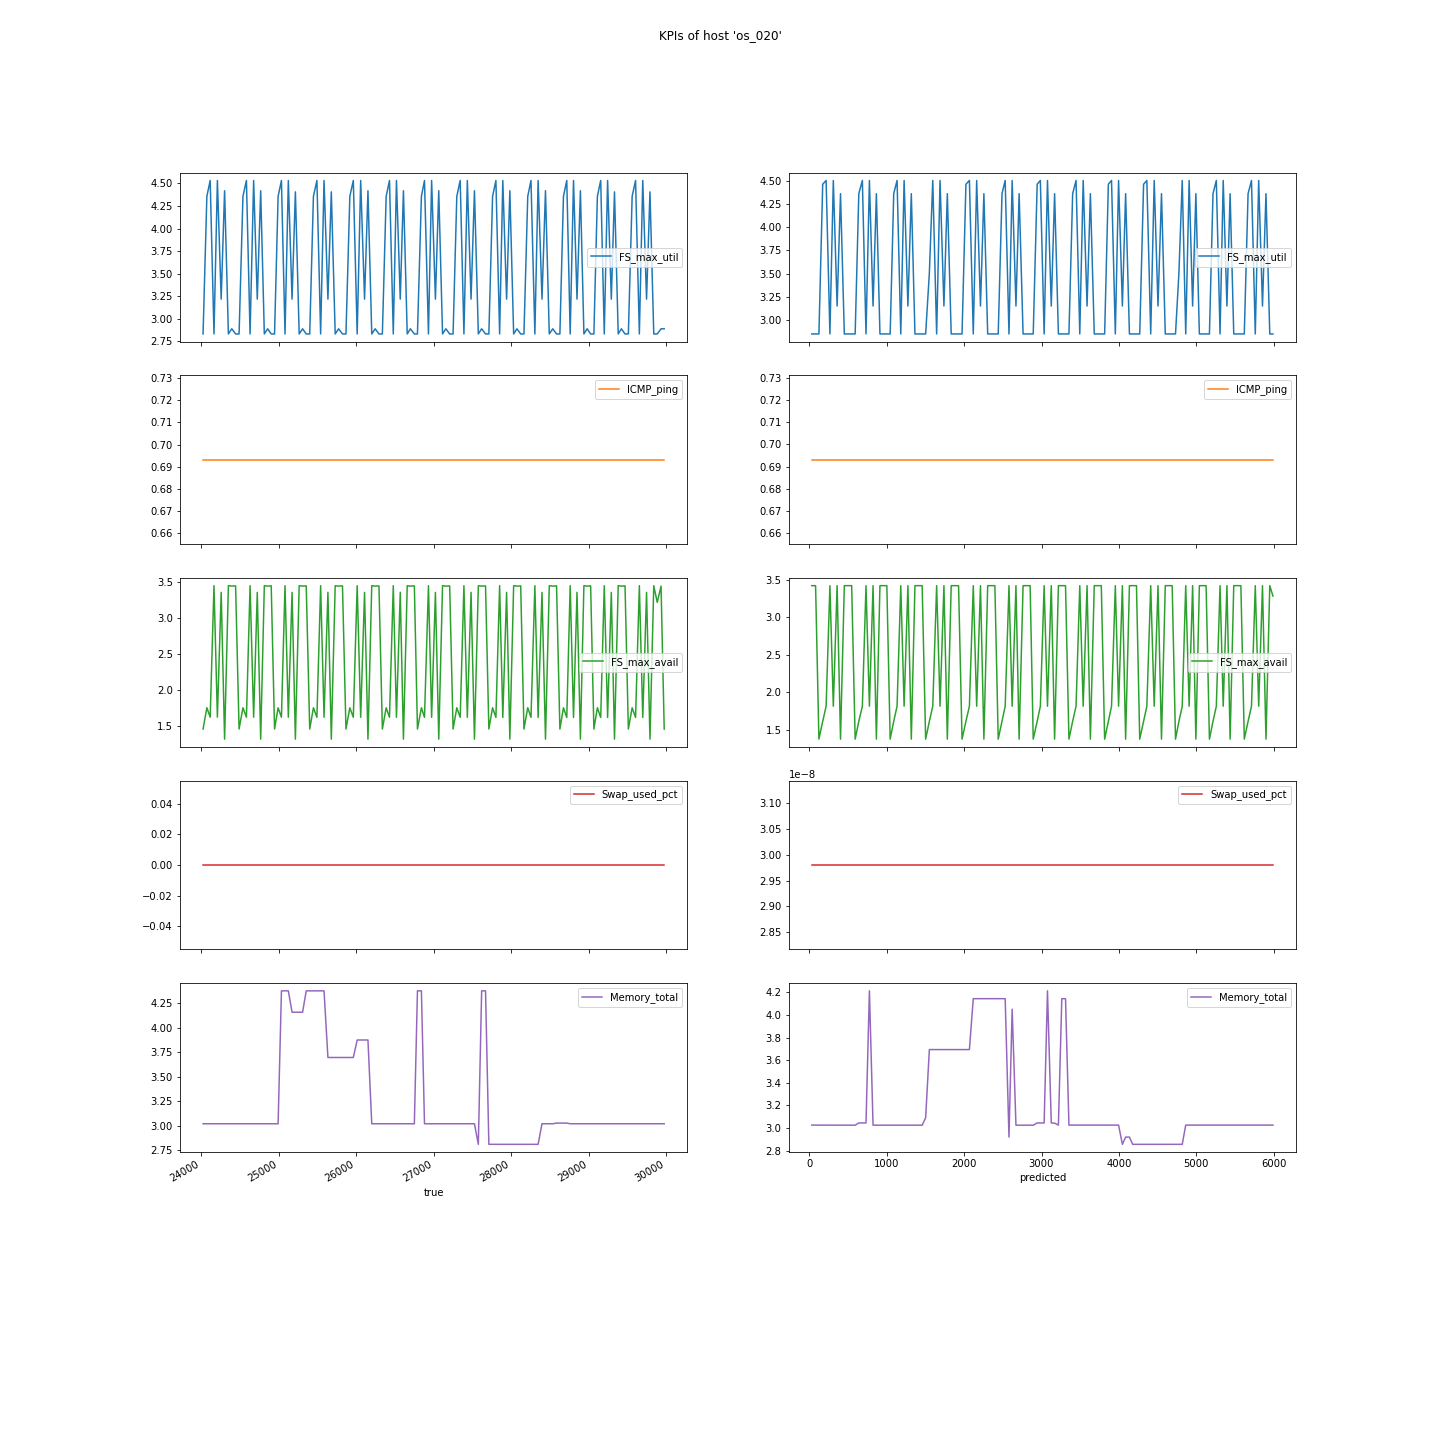
\includegraphics[width=0.5\textwidth]{images/multioutput_xgboost_os020.png}
  \caption{Sample of Multioutput xgboost forecasting KPIs of $os020$ (true/predicted)}
  \label{fig:xgboost}
\end{figure}


\end{document}
\endinput
%%
%% End of file `sample-acmsmall-conf.tex'.
